%{\setbeamercolor{background canvas}{bg=felix_bg}

\begin{frame}[t]
	\frametitle{Gerrymandering}

	\begin{center}
		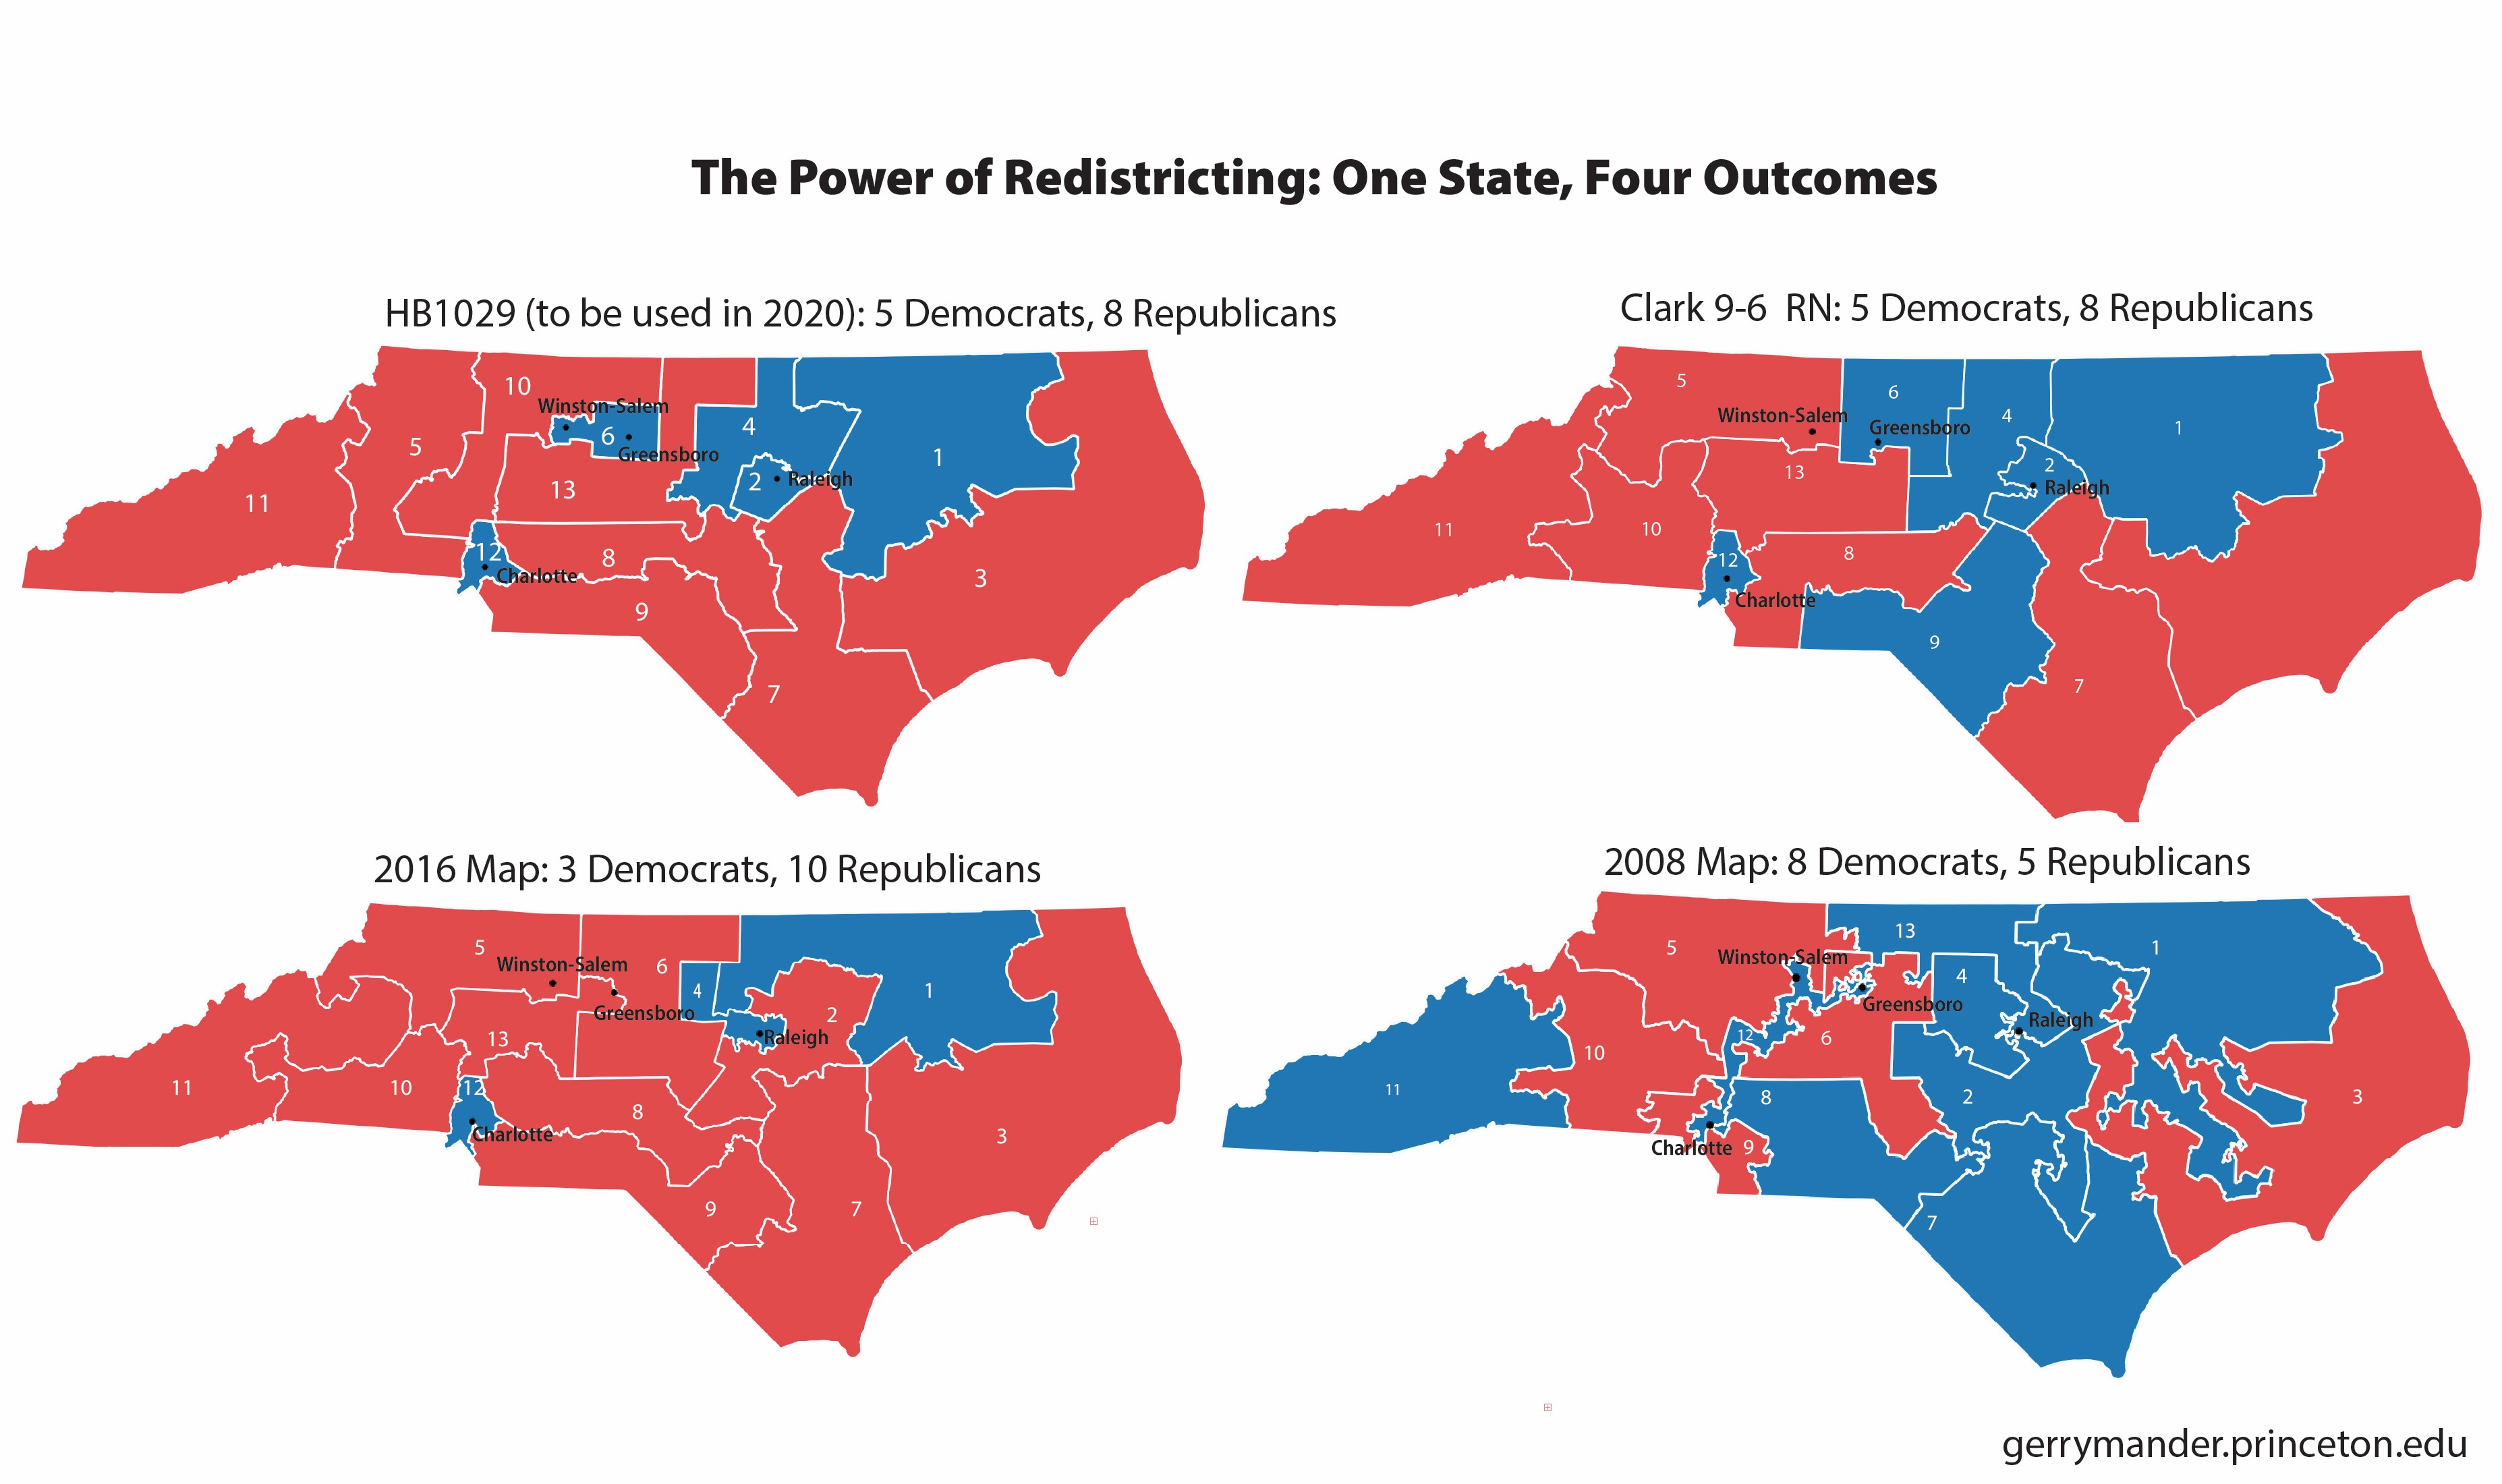
\includegraphics[width=\textwidth]{figures/NC_gerrymandering.jpg}
	\end{center}

	{\let\thefootnote\relax\footnote{{Source: election.princeton.edu}}}
\end{frame}

\begin{frame}[t]
	\frametitle{Gerrymandering on Graphs}
	\small
	\problembox{Gerrymandering}
	{A graph $G = (V,E)$, a set of candidates $C$, a candidate function $\chi: V \rightarrow C$, a weight function $w: V \rightarrow \mathbb{N}$, \only<1>{a preferred candidate $p \in C$, and an integer $k \in \mathbb{N}$.}\only<2>{\textcolor{red}{a preferred candidate $p \in C$, and an integer $k \in \mathbb{N}$.}}}
	{Is there a district-partition of $V$ into $k$ districts such that $p$ wins more districts than any other candidate?}

	\begin{figure}
		\begin{center}
			
\begin{tikzpicture}
	\tikzstyle{node} = [circle, draw, thick]
	\tikzstyle{edge} = [thick]

	\node (1) [node, fill=orange] {4};
	\node (2) [node, fill=orange, right=0.6cm of 1] {2};
	\node (3) [node, fill=skyblue, right=0.6cm of 2] {5};
	\node (4) [node, fill=orange, above=0.5cm of 2] {2};

	\node (5) [node, fill=bluegreen, below right=0.45cm and 0.3cm of 3] {3};
	\node (6) [node, fill=bluegreen, below right=0.5cm and 0.2cm of 1] {1};
	\node (12) [node, fill=bluegreen, below right=0.5cm and 0.2cm of 5] {7};

	\node (9) [node, fill=skyblue, below left=0.5cm and 0.2cm of 1] {4};
	\node (10) [node, fill=skyblue, below left=0.5cm and 0.1cm of 9] {2};
	\node (11) [node, fill=orange, below right=0.5cm and 0.1cm of 9] {5};

	\draw (1) edge [edge] (4);
	\draw (1) edge [edge] (6);
	\draw (1) edge [edge] (9);
	\draw (2) edge [edge] (4);
	\draw (3) edge [edge] (5);
	\draw (3) edge [edge] (4);

	\draw (9) edge [edge] (10);
	\draw (11) edge [edge] (9);
	\draw (12) edge [edge] (5);

	\tikzstyle{node} = []
\end{tikzpicture}

		\end{center}
	\end{figure}
\end{frame}

\begin{frame}[t]
	\frametitle{Gerrymandering Example}
	\begin{figure}
		\begin{center}
			
\begin{tikzpicture}
	\tikzstyle{node} = [circle, draw, thick]
	\tikzstyle{edge} = [thick]

	\node (1) [node, fill=orange] {4};
	\node (2) [node, fill=orange, right=0.6cm of 1] {2};
	\node (3) [node, fill=skyblue, right=0.6cm of 2] {5};
	\node (4) [node, fill=orange, above=0.5cm of 2] {2};

	\node (5) [node, fill=bluegreen, below right=0.45cm and 0.3cm of 3] {3};
	\node (6) [node, fill=bluegreen, below right=0.5cm and 0.2cm of 1] {1};
	\node (12) [node, fill=bluegreen, below right=0.5cm and 0.2cm of 5] {7};

	\node (9) [node, fill=skyblue, below left=0.5cm and 0.2cm of 1] {4};
	\node (10) [node, fill=skyblue, below left=0.5cm and 0.1cm of 9] {2};
	\node (11) [node, fill=orange, below right=0.5cm and 0.1cm of 9] {5};

	\draw (1) edge [edge] (4);
	\draw (1) edge [edge] (6);
	\draw (1) edge [edge] (9);
	\draw (2) edge [edge] (4);
	\draw (3) edge [edge] (5);
	\draw (3) edge [edge] (4);

	\draw (9) edge [edge] (10);
	\draw (11) edge [edge] (9);
	\draw (12) edge [edge] (5);

	\tikzstyle{node} = []

	\onslide<2-3> {
		\node (phint) [node, text=skyblue, above left=0.8cm and 0.3cm of 10] {$p$: 6 votes};
		\node (ohint) [node, text=orange, above left=0.4cm and 0.3cm of 10] {orange: 5 votes};
		\node (distresult) [node, above left=0cm and 0.3cm of 10] {$p$ wins!};
		\draw[ultra thick, rounded corners=6mm, color=skyblue] ($(9.north)+(0,0.5)$) -- ($(10.south west)+(-0.5,-0.2)$) -- ($(11.south east)+(0.5,-0.2)$) -- cycle;
	}

	\onslide<3> {
		\draw[ultra thick, rotate=-55, rounded corners, color=orange] ($(1.north west)+(-0.1,0.45)$) rectangle ($(6.south east)+(0.1, -0.45)$);

		\draw[ultra thick, rounded corners=10mm, color=skyblue] ($(4.north west)+(-0.1,0.7)$) -- ($(2.south west)+(-0.4,-0.4)$) -- ($(3.south east)+(0.7,-0.1)$) -- cycle;

		\draw[ultra thick, rotate=-55, rounded corners, color=bluegreen] ($(5.north west)+(-0.1, 0.45)$) rectangle ($(12.south east)+(0.1, -0.45)$);
	}
	
	

\end{tikzpicture}

		\end{center}
	\end{figure}

	\begin{itemize}
		\item Candidates $\rightarrow$ color. Our preferred candidate $p$ is blue.
		\item Weights $\rightarrow$ votes.
		\onslide<3> {
			\item Our candidate $p$ wins twice, others win once. Therefore, this is a YES-instance.
			\item This instance has $k=4$ districts.
		}
	\end{itemize}
\end{frame}

\begin{frame}[t]
	\frametitle{Parameterized Complexity}
	What if our problem considers an additional parameter $k$ such that $n >> k$?
	\vspace{1.0cm}
	\begin{itemize}
		\item FPT: There exists an algorithm that runs in $f(k)n^{O(1)}$ time.
		\vspace{1.0cm}
		\item W[2]-Hard: Most likely, no FPT algorithm exists.
		\vspace{1.0cm}
		\item XP: There exists an algorithm that runs in $n^{f(k)}$ time.
	\end{itemize}
\end{frame}